\chapter{狭义相对论：参考系、同时性与洛伦兹变换}

相对性原理是指物理定律不依赖于我们用来描述它们的惯性参考系。我们的首要任务是运动学：空间、时间、运动、同步以及从一个惯性系到另一个惯性系的变换的含义。动力学随后而来，包括相对论能量、动量、力、牛顿运动方程的类比，以及\(E=mc^2\)的含义。一旦这个结构稳固，我们就可以通过弯曲时空、粒子在给定引力场中的运动、黑洞以及宇宙膨胀，从概念上接近广义相对论，而不必从求解爱因斯坦场方程这一困难问题开始。

概念严谨性与数学严谨性之间的区别值得指出。我们不会使用明知是错误的近似。相反，我们将强调引力场对时钟、粒子和几何做了什么，同时推迟构造场方程任意解所需的工具。狭义相对论必须更明确地处理，因为所有后续推理都建立在其运动学之上。

因此，正确的起点不是某个著名的公式，而是精确说明观察者所说的位置和时间意味着什么。

\section{参考系是物理坐标系}

想象空间中充满了一个任意精细的米尺晶格。每个晶格点由三个空间坐标标记，并且在每个点都有一个时钟。这些杆和时钟共同构成了一个参考系。

\begin{definition}
一个\emph{事件}是在一个位置和一个时间发生的事情。在一维空间中，其坐标写作\((x,t)\)；在三维空间中，它们是\((x,y,z,t)\)。
\end{definition}

牛顿物理学增加了一个强有力的假设：所有理想时钟都可以一劳永逸地同步。时间是普适的。时钟可以被移动，观察者可以携带手表，但每个人都被认为在任何地方都同意同一个\(t\)。这有时被称为绝对时间；可以将其想象为上帝的时间，一个为整个世界服务的时钟。

相对性原理比爱因斯坦更古老。其自然的图景是一列在完美光滑的轨道上如此均匀地行驶的火车，以至于没有任何嘎嘎声或震动。在火车内部，我们可以像在停在车站的火车里一样抛接球。杂耍是一个令人惊讶地完整的小型力学实验：它需要计时、重力、对齐以及对轨迹的反复控制。如果火车以恒定速度行驶，这些规则都不会改变。竖直向上抛出的球会回到同一只手中；火车不会从它下面滑走。伽利略认识到了这一事实，牛顿在他的运动定律中系统地表达了它。

在伽利略之前，人们很容易推理说，移动的火车应该在球在空中时前进，迫使杂耍者向后或向前伸手去接它。错误在于忘记了球离开手时已经具有火车的水平速度。没有任何局限于平稳移动车厢内的实验能揭示绝对静止的特殊状态。只有两列火车之间的相对运动是可观察的。

因此，静止的火车和匀速运动的火车是两个惯性系。在爱因斯坦之前，它们通过伽利略变换相关联。

\section{绘制时空图}

我们暂时忽略\(y\)和\(z\)，将时间竖直绘制，位置\(x\)水平绘制。图中的每个点都是一个事件。线\(x=0\)是空间原点的历史，或\emph{世界线}。相邻的竖直线\(x=1,2,3,\ldots\)是其他晶格点的世界线。水平线是具有共同时间的事件集合。

\begin{figure}[H]
\centering
\includegraphics[width=0.62\textwidth]{lecture_01_figure_02.png}
\caption{静止参考系的时间轴和空间晶格的第一批世界线。}
\lectureframe{00:16:38}
\end{figure}

同样的构造在理想化图中更清晰：

\begin{figure}[H]
\centering
\begin{tikzpicture}[scale=0.95]
\draw[->] (-1.2,0) -- (5.2,0) node[right] {$x$};
\draw[->] (0,-0.2) -- (0,4.8) node[above] {$t$};
\foreach \x in {-1,1,2,3,4}
  \draw[gray!65] (\x,0) -- (\x,4.4);
\foreach \y in {1,2,3,4}
  \draw[gray!65] (-1.0,\y) -- (4.4,\y);
\fill (0,0) circle (1.5pt);
\node[below left] at (0,0) {$0$};
\node[left] at (0,1) {$1$};
\node[left] at (0,2) {$2$};
\node[left] at (0,3) {$3$};
\node[below] at (1,0) {$1$};
\node[below] at (2,0) {$2$};
\node[below] at (3,0) {$3$};
\end{tikzpicture}
\caption{一个静止的时空晶格。竖直线具有恒定位置；水平线具有恒定时间。}
\end{figure}

网格是想象的，其间距是任意的。我们可以使用米、厘米、微米或任何更小且具有物理意义的间隔。其目的是为每个事件分配精确的坐标。

“参考系”这个说法现在有了可操作的内容。它不仅仅是一个视角，或某个朝某个方向看的人。它是一个延展的坐标装置。给定一个事件，当地的尺子指明它发生在哪里，当地的钟指明它发生在何时。于是其他物理量就可以在不同参考系之间进行比较：一个粒子的位置和速度、它的能量、也许还有一个物体的温度，最终还有它的动量和力。最简单的比较是涉及\(x\)和\(t\)的那一种，所以我们就从那里开始。

现在，在一列沿\(x\)正方向以恒定速度\(v\)行驶的火车上放置第二套格点。选择两原点在\(t=0\)时重合。于是运动的原点遵循
\begin{equation}
x=vt.
\end{equation}
固定在火车上的其他每一个点都遵循一条平行的倾斜世界线。这种倾斜不过是如下几何陈述：火车随时间推移而改变位置。

假设火车尾部的点是带撇原点。在\(t=0\)时，它与车站原点重合。在较晚的时刻\(t\)，它的静止坐标为\(vt\)。因此，一个位于坐标\(x\)附近的事件距离火车原点只有\(x-vt\)。这就是为什么该变换是一次减法，而不是一条任意的代数规则。

设\((x,t)\)为一个事件在车站系中的坐标，\((x',t')\)为它在火车系中的坐标。伽利略和牛顿保留普适时间，
\begin{equation}
t'=t.
\end{equation}
在时间\(t\)内，运动的原点前进\(vt\)，所以从该原点到该事件的距离为
\begin{equation}
x'=x-vt.
\end{equation}
合起来，
\begin{align}
t'&=t, & x'&=x-vt.
\label{eq:galilean-forward}
\end{align}
解出不带撇的坐标，就得到逆变换，
\begin{align}
t&=t', & x&=x'+vt'.
\label{eq:galilean-inverse}
\end{align}

\begin{figure}[H]
\centering
\includegraphics[width=0.72\textwidth]{lecture_01_figure_03.png}
\caption{与两个时空格点并列写出的伽利略变换。}
\lectureframe{00:21:57}
\end{figure}

第一对公式告诉运动的观察者如何转换静止观察者提供的坐标。逆变换那一对则转换回去。这种在两种描述之间的相互转换，就是伽利略相对论的数学内容。

在逆空间公式中作替换\(t\to t'\)之所以无害，只是因为伽利略理论已经宣告了\(t=t'\)。现在注意到这个假设是有益的。在爱因斯坦的理论中，两个时间坐标将不同，而这样的替换将不再是自动成立的。

\begin{classroomqa}
\audiencequestion{如果一只钟被带走，然后又被带回来，我们怎么能知道它的运动没有先使它变快、然后又使它变慢，从而在比较这些钟时把效应掩盖起来呢？
\lecturetimestamp{00:23:09}}
\lecturerresponse{伽利略不可能以现代精度确立普适时间；那是一个物理猜测。我们可以用许多方式检验这个猜测：把好钟沿相反方向携带，把北--南之行以及东--西之行都重复，让一只钟绕另一只钟运动，或者在不把钟放在一起的情况下交换授时信号。在普通速度下，所有这类检验都以极高精度一致。有了足够精确的钟，或者足够大的速度，就会出现一个微小的偏差。普适时间的这种失效并不是实验的缺陷；它是狭义相对论必须解释的现象之一。}
\end{classroomqa}

\section{伽利略不变量与牛顿定律}

不变量是所讨论的所有惯性观察者都同意的一个量。坐标本身不必是不变量。要紧的是，由它们组装出来的定律是否保持相同的形式。

这个词既用作名词，也用作形容词。一个数可以是不变量，而一个方程可以在某个变换下是不变的。不变量与不变定律之间的区分防止了一种常见的混淆：相对论并不主张每个观察者对一切事物都得到相同的坐标。它主张的是，联系他们测量结果的物理定律具有相同的形式。

取两个同时发生的事件，位置分别为\(x_1\)和\(x_2\)。方程~\eqref{eq:galilean-forward}给出
\begin{align}
x_1'&=x_1-vt,\\
x_2'&=x_2-vt.
\end{align}
因此它们的间隔为
\begin{equation}
x_2'-x_1'=(x_2-vt)-(x_1-vt)=x_2-x_1.
\end{equation}
在伽利略物理学中，同时发生的事件之间的距离是不变量，尽管各个位置本身不是。

\begin{classroomqa}
\audiencequestion{那个减法中出现的两个\(t\)真的是同一个时间吗？
\lecturetimestamp{00:28:16}}
\lecturerresponse{是的。我们特意选择这两个事件为\((x_1,t)\)和\((x_2,t)\)。它们位于同一条水平的等时线上。因此公共项\(vt\)相消。如果这些事件发生在不同时间，这个论证就不会确立一个不变的空间间隔。}
\end{classroomqa}

现在用轨迹\(x(t)\)描述一个粒子。列车观察者给出
\begin{equation}
x'(t)=x(t)-vt.
\end{equation}
求一次导数便得到熟悉的速率相加法则，
\begin{equation}
\frac{dx'}{dt}=\frac{dx}{dt}-v.
\end{equation}
位置和速率依赖于参考系。与一支箭并排运动的观察者看到它行进得比站在轨道旁的观察者更慢。

再求一次导数。由于相对速率\(v\)是常量，
\begin{equation}
\frac{d^2x'}{dt^2}=\frac{d^2x}{dt^2}.
\end{equation}
加速度在伽利略变换下不变。这有力地提示了为什么牛顿定律用加速度而不是位置或速率来书写。

这是被观测物体的加速度，而不是列车观察者的加速度。两个参考系都是惯性的，因此两个参考系彼此之间都不加速。物体在任一种描述中都可能向左或向右加速，而两个观察者对该加速度的数值一致，尽管他们对物体的位置和速率并不一致。

假设两个粒子彼此施加一个力，且该力只依赖于它们在同一时刻的间距。该间距是不变量，因此该力也是不变量。如果质量同样是一种内禀的、与参考系无关的性质，那么每个惯性观察者都能以完全相同的形式写出
\begin{equation}
F=ma
\end{equation}
牛顿力学在伽利略变换下不变。这不仅仅看似合理；在通常速率的整个范围内，它都极其精确。

该论证适用于熟悉的有心力，例如牛顿引力或静电作用，其中大小是距离的函数。由于所有伽利略观察者在同一时刻对该距离一致，他们对该力也一致。在力和加速度都确定的情况下，一致性进而要求他们对质量也一致：一个1千克的物体被列车带过时仍然是一个1千克的物体。\(F=ma\)中的每个符号都符合同样的不变结构。

\section{光不符合伽利略法则}

电磁学造成了困难。麦克斯韦方程组预言波以确定速率\(c\)穿过真空传播。如果麦克斯韦方程组是自然定律，而自然定律在每个惯性参考系中都相同，那么所有惯性观察者都必须得到相同的\(c\)。

伽利略运动学预言了别的东西。在静止参考系中向右运动的光脉冲满足
\begin{equation}
x=ct.
\end{equation}
施加空间变换得到
\begin{equation}
x'=x-vt=(c-v)t.
\end{equation}
由于\(t'=t\)，列车观察者将测得速率\(c-v\)。

这一矛盾可以尖锐地陈述出来。如果麦克斯韦方程组保持其形式，它们就在带撇参考系中预言\(c\)。如果保留伽利略变换，它就预言\(c-v\)。当\(v\ne0\)时，两者不可能都精确成立。

如果光在介质中的行为像普通波，这个结果看起来就完全自然。随水波运动的船测得较低的相对波速。在静止空气中运动的听者测得的声速会因听者相对于空气的运动而发生偏移。因此，19世纪的物理学家被引向一个优先的静止状态，即一个以太参考系，在其中麦克斯韦方程组具有其最简单形式，而光以\(c\)运动。旨在探测相对于这样一个优先参考系的运动的实验没有发现相应的效应。

有若干种可能的实验安排，但它们的共同目标是比较处于不同运动状态或方向的观察者所看到的光传播。没有一个实验揭示出预期的伽利略偏移。这一失败并不是小小的技术麻烦。它迫使人们在相对性原理、麦克斯韦方程组以及继承下来的空间和时间观念之间做出选择。

爱因斯坦更直接地处理这一冲突。年轻时，他想象追逐一列光波。如果他能追上它，它振荡的电磁图样就会冻结在空间中，然而麦克斯韦方程组不允许这样的静止光波。他选择把麦克斯韦理论和相对性原理视为基本的，然后重新审视隐藏在我们的坐标中的假设。

这一重建基于两条公设：
\begin{enumerate}
\item 物理定律在每个惯性参考系中都具有相同的形式。
\item 真空中的光在每个惯性参考系中都具有相同的速率\(c\)。
\end{enumerate}

第二条公设不能与伽利略变换共存。某种比速度相加法则更深层的东西必须改变。爱因斯坦的简洁选择是保留这两条公设，并重新审视那个看似无害的伽利略方程\(t'=t\)。

\section{同步远处的钟}

空间距离可以用杆来铺设，但远处的钟需要一种同步约定。把两个钟放在与中点观察者等距的位置。当每个端点处的钟读到约定时刻时，让它发出一次闪光。如果两次闪光同时到达中点，就称端点处的钟已同步。如果一次闪光先到达，就调整相应的钟并重复该程序。

“\emph{中点}”一词是用该参考系中已经铺设好的杆来定义的。因此这个检验包含两个彼此独立的要素：到两端点的空间距离相等，以及信号到达时间相等。两个要素都不能省略。在整个格点上重复该程序，就提供了牛顿曾直接假定的水平等时线。

这个定义使用光，是因为该公设赋予光在每个惯性系中相同的速度。一旦所有相邻的钟对都按这种方式处理完毕，整个格点就带有一族同步的钟。

现在让第二个格点穿过第一个格点运动。运动装置的中点在它自己的参考系中仍位于两个运动端点之间的中点。然而，相对于静止装置，它朝着一束迎面而来的闪光运动，并远离另一束闪光。按照静止钟同时发出的闪光，并不会同时到达运动的中点。由于运动的观察者应用同样的中点与光规则，该观察者不能称那些发射是同时的。每个参考系都一致地同步自己的钟，但这两个同步方案并不一致。

这并不是由光的有限传播时间造成的光学错觉。每个观察者都知道光需要时间才能到达，并用相同的速度\(c\)对此进行修正。修正之后分歧仍然存在，因为观察者并不会把同样的远处事件选为一对同时事件。相对的正是同时性本身，而不只是同时性的表象。

\begin{classroomqa}
\audiencequestion{我们能否改用声音而不是光来同步钟，从而避免这个结论？
\lecturetimestamp{00:49:03}}
\lecturerresponse{在空气静止的参考系中，声音可以作为同步信号，但在每个惯性系中测得的声音速度并不相同。一列穿过静止空气的敞篷列车相对于传声介质在运动，因此向前和向后的声音信号在那里并不对称。光按公设则不同：不存在可探测的光学介质，其静止参考系会选出一个观察者。因此我们使用光，并遵循其后果。}
\end{classroomqa}

定性上的分歧已经清楚。现在我们来精确计算运动观察者称哪些事件为同时事件。

\section{光线的构造}

为了进行构造，方便的做法是选择如下单位：
\begin{equation}
c=1.
\end{equation}
于是，一个距离单位就是光在一个时间单位内走过的距离：光秒与秒配对，或光年与年配对。空间和时间带有相同的单位，速度是无量纲的，光线出现在\(45^\circ\)处。向右运动的光线有
\begin{equation}
x=t+d,
\end{equation}
而向左运动的光线有
\begin{equation}
x=-t+d'.
\end{equation}
过原点的两条光线就分别是\(x=t\)和\(x=-t\)。属于比光慢的物体的类时轨迹，更靠近竖直轴。假设的超光速轨迹则会更靠近水平轴。

图中的角度只有在这种单位选择之后才有意义。若用米和秒，光线看起来几乎水平，因为它在1秒内大约走过\(3\times10^8\)米。选择光秒作为距离会重新标定水平轴，并使因果几何变得可见。

考虑运动格点中的三条平行世界线，
\begin{equation}
x=vt,\qquad x=vt+L,\qquad x=vt+2L.
\label{eq:moving-worldlines}
\end{equation}
中间的世界线属于那个检验两个外侧点之间同时性的观察者。这三个点都匀速运动，并在带撇参考系中保持它们的相对排列。

\begin{figure}[H]
\centering
\includegraphics[width=0.72\textwidth]{lecture_01_figure_04.png}
\caption{向右的光线\(x=t\)与中间运动世界线相交。}
\lectureframe{01:02:33}
\end{figure}

完整的几何可以画出来，而不必受站在黑板前的人的妨碍：

\begin{figure}[H]
\centering
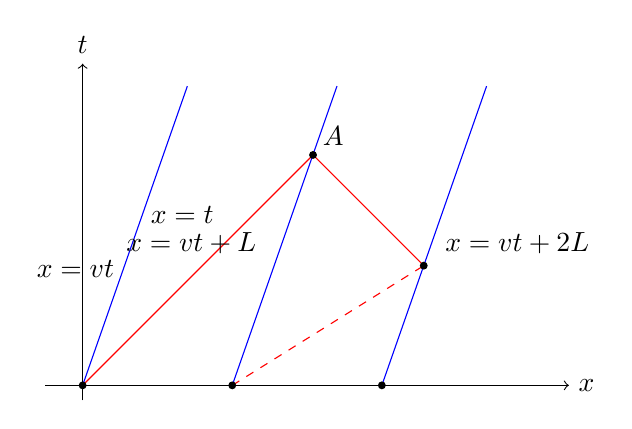
\begin{tikzpicture}[scale=0.95]
\draw[->] (-0.5,0) -- (6.5,0) node[right] {$x$};
\draw[->] (0,-0.2) -- (0,4.3) node[above] {$t$};
\draw[blue] (0,0) -- (1.4,4.0);
\draw[blue] (2.0,0) -- (3.4,4.0);
\draw[blue] (4.0,0) -- (5.4,4.0);
\draw[red] (0,0) -- (3.08,3.08);
\draw[red] (3.08,3.08) -- (4.56,1.60);
\draw[red,dashed] (2.0,0) -- (4.56,1.60);
\fill (0,0) circle (1.5pt);
\fill (2.0,0) circle (1.5pt);
\fill (4.0,0) circle (1.5pt);
\fill (3.08,3.08) circle (1.5pt);
\fill (4.56,1.60) circle (1.5pt);
\node[left] at (0.55,1.55) {$x=vt$};
\node[left] at (2.45,1.9) {$x=vt+L$};
\node[right] at (4.72,1.9) {$x=vt+2L$};
\node[left] at (1.88,2.28) {$x=t$};
\node[above right] at (3.08,3.08) {$A$};
\end{tikzpicture}
\caption{光信号决定运动参考系的等时线。}
\end{figure}

从原点发出一束向右运动的光线。设\(A\)为它与中间世界线的交点。\(A\)处的两个方程是
\begin{align}
x&=t,\\
x&=vt+L.
\end{align}
代入得到
\begin{equation}
t=vt+L,
\end{equation}
因此
\begin{equation}
t_A=x_A=\frac{L}{1-v}.
\label{eq:point-a}
\end{equation}

从\(A\)出发，沿一条向左运动的光线反向追溯到最右侧的运动世界线。其方程具有如下形式
\begin{equation}
x+t=b.
\end{equation}
由于它经过\(A\)，方程~\eqref{eq:point-a}确定了常数：
\begin{equation}
b=x_A+t_A=\frac{2L}{1-v}.
\end{equation}
因此这条反向光线满足
\begin{equation}
x+t=\frac{2L}{1-v}.
\label{eq:backward-ray}
\end{equation}

它与最右侧世界线的交点可由下式得到
\begin{align}
x+t&=\frac{2L}{1-v},\\
x&=vt+2L.
\end{align}
消去\(x\)，
\begin{align}
(1+v)t
  &=2L\left(\frac{1}{1-v}-1\right)\\
  &=\frac{2Lv}{1-v},
\end{align}
所以
\begin{equation}
t=\frac{2Lv}{1-v^2}.
\end{equation}
代入\(x=vt+2L\)得到
\begin{equation}
x=\frac{2L}{1-v^2}.
\end{equation}
坐标本身不如它们的比值重要：
\begin{equation}
\frac{t}{x}=v.
\end{equation}
因此，按照运动时钟与原点同时的每一个事件都位于
\begin{equation}
t=vx,
\label{eq:simultaneity-c-one}
\end{equation}
而运动的原点则沿
\begin{equation}
x=vt.
\label{eq:moving-time-axis}
\end{equation}
这两条轴关于\(45^\circ\)光线对称地倾斜。

\(x=vt\)上的所有点都具有相同的带撇位置，\(x'=0\)，而它们的带撇时间各不相同。\(t=vx\)上的所有点都具有相同的带撇时间，\(t'=0\)，而它们的带撇位置各不相同。因此，其中一条线是带撇时间轴，另一条是带撇空间轴。需要借助长信号构造来确定第二条线；仅凭运动世界线无法推断出它。

在方程~\eqref{eq:simultaneity-c-one}中恢复普通单位需要
\begin{equation}
t=\frac{v}{c^2}x.
\label{eq:simultaneity-dimensional}
\end{equation}
因子\(c^2\)解释了为什么牛顿图像在日常生活中如此有效。对于远小于\(c\)的速度，运动同时线的斜率极小。

\begin{figure}[H]
\centering
\includegraphics[width=0.72\textwidth]{lecture_01_figure_05.png}
\caption{当\(c=1\)时，带撇时间轴与同时轴关于光线对称。}
\lectureframe{01:15:40}
\end{figure}

\begin{figure}[H]
\centering
\begin{tikzpicture}[scale=1.0]
\draw[->] (-2.2,0) -- (5.2,0) node[right] {$x$};
\draw[->] (0,-0.2) -- (0,4.9) node[above] {$t$};
\draw[red] (0,0) -- (3.9,3.9);
\draw[red] (0,0) -- (-1.8,1.8);
\draw[blue] (0,0) -- (1.8,4.5);
\draw[blue,dashed] (0,0) -- (4.5,1.8);
\node[right] at (3.9,3.9) {$x=t$};
\node[left] at (-1.8,1.8) {$x=-t$};
\node[above] at (1.8,4.5) {$x'=0$};
\node[right] at (4.5,1.8) {$t'=0$};
\end{tikzpicture}
\caption{以\(c=1\)为单位的带撇轴与不变光线。}
\end{figure}

\section{推导洛伦兹变换}

几何结构确定了每个带撇坐标在何处为零。沿运动时间轴\(x=vt\)，必须有\(x'=0\)。沿运动同时轴\(t=vx\)，必须有\(t'=0\)。具有这些零集的最一般线性关系可以写成
\begin{align}
x'&=\frac{x-vt}{F(v)},\\
t'&=\frac{t-vx}{G(v)}.
\label{eq:fg-ansatz}
\end{align}
因子\(F\)和\(G\)允许带撇坐标的标度不同于伽利略标度，即使两条轴的位置已经确定。线性来自空间和时间的均匀性：平移一个实验不可能改变变换律。\editorialnote{这个简短的线性论证明确指出了黑板推导中隐含使用的一个假设。}

在这个阶段，几何已经告诉了我们很多，但并非全部。分子确定了轴的倾斜。它们并未确定沿这些轴的单位间距。那部分剩余的标度信息正是\(F(v)\)和\(G(v)\)所表示的。

现在施加光速不变性。一条满足\(x=t\)的向右运动光线也必须满足\(x'=t'\)。沿这条光线，
\begin{align}
x'&=\frac{(1-v)t}{F(v)},\\
t'&=\frac{(1-v)t}{G(v)}.
\end{align}
对光线上每一点都相等要求
\begin{equation}
F(v)=G(v).
\end{equation}
因此我们可以写出
\begin{align}
x'&=\frac{x-vt}{F(v)},\\
t'&=\frac{t-vx}{F(v)}.
\label{eq:common-f}
\end{align}

这一步在代数中使用了第一个真正属于爱因斯坦的要求。同一条几何直线对两个观察者都是光线，因此当\(c=1\)时，沿它两个带撇坐标必须等量增加。若两个方程中的因子不同，带撇速度就会不等于1。

还剩一个未知函数。将方程~\eqref{eq:common-f}乘以\(F(v)\)：
\begin{align}
F(v)x'&=x-vt,\\
F(v)t'&=t-vx.
\end{align}
将第二个方程乘以\(v\)并与第一个相加，消去\(t\)，得到
\begin{equation}
(1-v^2)x=F(v)(x'+vt').
\end{equation}
类似地，
\begin{equation}
(1-v^2)t=F(v)(t'+vx').
\end{equation}
因此逆变换为
\begin{align}
x&=\frac{F(v)}{1-v^2}(x'+vt'),\\
t&=\frac{F(v)}{1-v^2}(t'+vx').
\end{align}

相对性原理使两个参考系互为对等。如果车站看到列车以\(+v\)运动，那么列车看到车站以\(-v\)运动。因此，逆方程必须与正方程具有相同形式，只是\(v\)的符号相反。它们的前置因子必须满足
\begin{equation}
\frac{F(v)}{1-v^2}=\frac{1}{F(v)}.
\end{equation}
因此
\begin{equation}
F(v)^2=1-v^2,
\end{equation}
而在\(v=0\)处与恒等变换的连续性选出正根，
\begin{equation}
F(v)=\sqrt{1-v^2}.
\end{equation}

没有任何东西是针对某个特定光脉冲拟合出来的。这个结果来自由同步确定的两条轴、共同的光速，以及要求两个惯性系都不比另一个更特殊。

在\(c=1\)的单位制下，洛伦兹变换为
\begin{align}
x'&=\frac{x-vt}{\sqrt{1-v^2}},\\
t'&=\frac{t-vx}{\sqrt{1-v^2}}.
\label{eq:lorentz-c-one}
\end{align}
其逆变换为
\begin{align}
x&=\frac{x'+vt'}{\sqrt{1-v^2}},\\
t&=\frac{t'+vx'}{\sqrt{1-v^2}}.
\end{align}

\begin{figure}[H]
\centering
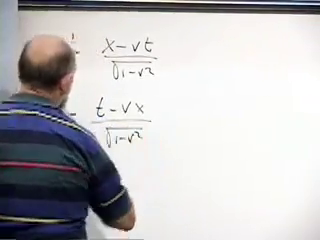
\includegraphics[width=0.76\textwidth]{lecture_01_figure_06.png}
\caption{黑板上完成的\(c=1\)洛伦兹变换。}
\lectureframe{01:32:38}
\end{figure}

本质上的新意已经在时间方程中显现出来。时间并不是简单地从一个参考系原样带到另一个参考系。带撇时间坐标混合了不带撇时间和位置。因此，\(t=\text{constant}\)和\(t'=\text{constant}\)描述的是不同的若干事件集合。

混合项并不是事后附加的可选修正。没有它，\(t'=0\) 这条线就会保持水平，异地同时性就会保持普适，而该变换也无法保持光速。

\section{恢复光速并检验结果}

当 \(c\ne1\) 时，量纲一致性会补回缺失的因子。比值 \(v^2/c^2\) 是无量纲的，而 \((v/c^2)x\) 具有时间的量纲。因此
\begin{align}
x'&=\frac{x-vt}{\sqrt{1-v^2/c^2}},\\
t'&=\frac{t-(v/c^2)x}{\sqrt{1-v^2/c^2}}.
\label{eq:lorentz-dimensional}
\end{align}
将 \(v\) 的符号反转，就得到逆变换：
\begin{align}
x&=\frac{x'+vt'}{\sqrt{1-v^2/c^2}},\\
t&=\frac{t'+(v/c^2)x'}{\sqrt{1-v^2/c^2}}.
\end{align}
引入
\begin{equation}
\gamma=\frac{1}{\sqrt{1-v^2/c^2}}
\end{equation}
会把这些式子写成熟悉的紧凑形式，但分母形式使推导过程保持可见。

数值上，\(c\simeq3\times10^8\,\mathrm{m/s}\)，所以 \(c^2\simeq9\times10^{16}\,\mathrm{m^2/s^2}\)。巨大的分母使得同时性倾斜和因子 \(v^2/c^2\) 在大多数力学实验中都难以察觉。它们的微小性解释了伽利略的成功；但这并不能恢复绝对时间。

\begin{figure}[H]
\centering
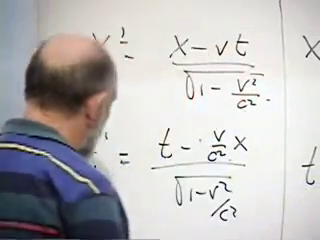
\includegraphics[width=0.76\textwidth]{lecture_01_figure_07.png}
\caption{恢复 \(c\) 的因子之后的洛伦兹变换。}
\lectureframe{01:35:58}
\end{figure}

两项检验立即可得。首先取 \(v\ll c\)。于是 \(v^2/c^2\) 可以忽略，而对于通常的距离，同时性相对性项 \(vx/c^2\) 也可以忽略。式~\eqref{eq:lorentz-dimensional} 化为
\begin{equation}
t'\approx t,\qquad x'\approx x-vt.
\end{equation}
伽利略相对性作为低速近似被重新得到。

其次，检验一条光线。一旦 \(c\) 被恢复，向右运动的光线满足 \(x=ct\)，而不是 \(x=t\)。代入给出
\begin{align}
x'&=\frac{(c-v)t}{\sqrt{1-v^2/c^2}},\\
t'&=\frac{(1-v/c)t}{\sqrt{1-v^2/c^2}}.
\end{align}
由于 \(c-v=c(1-v/c)\)，
\begin{equation}
x'=ct'.
\end{equation}
带撇的观察者测得相同的速率 \(c\)。对于向左运动的光线，代入 \(x=-ct\) 同样给出
\begin{equation}
x'=-ct'.
\end{equation}
该变换正确地处理了沿任一方向运动的光。

\(x=t\) 与 \(x=ct\) 之间的区别是一个有启发性的量纲检验。前者仅在 \(c=1\) 的单位制下才是正确的。如果在变换中恢复通常单位，却把光线方程留在自然单位中，就会混合两种约定并产生错误结果。量纲一致性会立刻抓住这个错误。

\section{中点判据}

\begin{classroomqa}
\audiencequestion{假设一个观察者在同一瞬间接收到两次闪光，但他并不位于两个光源之间的中点。这个观察者可以断定两次闪光是同时发出的吗？
\lecturetimestamp{01:42:55}}
\lecturerresponse{不可以。只有当观察者在相关参考系中空间上位于两个光源的正中间时，相同的到达时间才意味着相同的发射时间。一个更靠近某个光源的接收者可以同时接收到两次闪光，即使较远的那次闪光发射得更早。因此在运动构造中，中点世界线 \(x=vt+L\) 是必不可少的。向前光线 \(x=t\) 被追踪到它与该中点相遇，然后一条向后光线被追溯到 \(x=vt+2L\)。按照运动参考系，与原点同时的是第二个端点事件，而不是别处任意一个到达时间相同的事件。}
\end{classroomqa}

我们已经得到了完整的坐标变换，但还没有得到它最熟悉的推论。接下来是长度收缩、时间膨胀和固有时，然后是相对论动量和能量。基础已经就位：每个惯性系之所以可以使用相同的定律并测得相同的光速，只是因为空间和时间会混合，而且异地同时性属于某个参考系，而不是绝对地属于世界。